With the combined knowledge of the two last sections, the ground state (and the ground state energy) can be calculated. It will become evident, that the calculation is really simple to do and program. Sadly it won't be feasable to compute sufficiently large lattices, because of the exponential nature of the problem.

\begin{figure}[htbp]
    \centering
    \makebox[\textwidth][c]{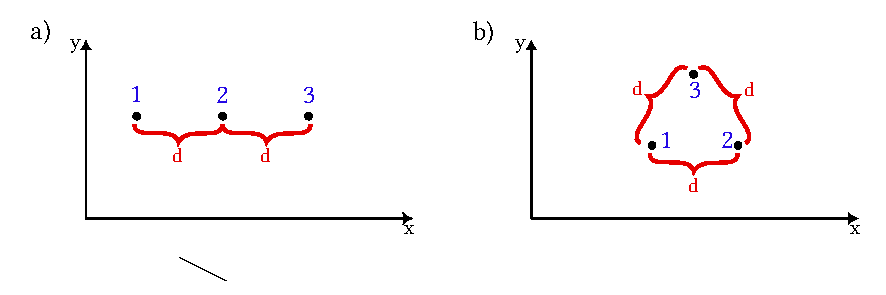
\includegraphics[width=0.9\textwidth]{./theory/physics/numerical-solutions/simple_case.pdf}}
    \vspace{-1cm}
    \caption{A representation of two simple latices. The spins are fixed at the point of the numbered locations. All sites have the same distance $d$ from each other. Note, that a spin up \up is directed parallel to the z-axis. That means in this case it would point out of the paper in the direction of the viewer.}
    \label{fig:simpleThreeLatticeIsing}
\end{figure}

In the beginning one trivial example will be discussed. The lattice is visualized in \autoref{fig:simpleThreeLatticeIsing}, image a).
This corresponds to a linear lattice in 1D. Let the Hamiltonian be the one in \autoref{eq:hamiltonianExampleA}.

\begin{equation}
    \label{eq:hamiltonianExampleA}
    \hamiltonian = \sigma^z_1\sigma^z_2 + \sigma^z_2\sigma^z_3
\end{equation}

This hamiltonian is anti-ferromagnetic ($J = +1$). It should be easily seen, that the Energy $E$ in \autoref{eq:schroedinger-general} becomes minimal (largest magnitude with negative sign) when the spins always point into the opposite direction as their neighbors: $\ket{\up, \down, \up}$ or $\ket{\down, \up, \down}$. This is quite a crucial step, so trying this by one self is advised for someone without prior quantum mechanical experience.
The ground state therefore will be a \emph{superposition} consisting of equal parts $\ket{\up, \down, \up}$ and $\ket{\down, \up, \down}$ (\autoref{eq:solutionSimpleExample}). The factor $\frac{1}{\sqrt[]{2}}$ instead of the seemingly more obvious $\frac{1}{2}$ makes the wavefunction be \emph{normalized}. If it wasn't for the square root, \autoref{eq:base-orthonormal} would not be satisfied. This way it is satisfied, which can be tested.

\begin{equation}
    \label{eq:solutionSimpleExample}
    \Psi_\mathrm{gnd} = \frac{1}{\sqrt[]{2}} \cdot \ket{\up, \down, \up} +  \frac{1}{\sqrt[]{2}} \cdot \ket{\down, \up, \down}
\end{equation}

The second example, visualized in \autoref{fig:simpleThreeLatticeIsing}, image b), however is not so simple. The corresponding hamiltonian can be seen in \autoref{eq:hamiltonianExampleB}.
\begin{equation}
    \label{eq:hamiltonianExampleB}
    \hamiltonian = \sigma^z_1\sigma^z_2 +\sigma^z_2\sigma^z_3 +\sigma^z_1\sigma^z_3
\end{equation}
It has one more interaction than the previous one. Even though it also is anti-symmetric, it is \emph{not} possible to align all three spins in a way, so that they stand anti-parallel to all their neighbors. This phenomenon is called \emph{frustration} \cite*{frustration}.

Already this minimal problem has a complex superposition of eight base states as a ground state. The introduction of the transverse field will only make this more complex. Therefore a systematic way of finding the solution will be presented.

For this purpose, the example from \autoref{fig:simpleThreeLatticeIsing}, image b) will be used once more, but this time with the hamiltonian in \autoref{eq:hamiltonianExampleTransverse}.
\begin{equation}
    \label{eq:hamiltonianExampleTransverse}
    \hamiltonian = J\cdot \sigma^z_1\sigma^z_2 +J\cdot\sigma^z_2\sigma^z_3 +J\cdot\sigma^z_1\sigma^z_3
    +h \sigma^x_1+h \sigma^x_2+h \sigma^x_3
\end{equation}

The goal is now, to write the hamiltonian \hamiltonian as a matrix. 
The elements of the matrix should be $\bra{m}\hamiltonian\ket{n}$. Where $\ket{m}$ and $\ket{n}$ are two states out of the chosen basis. In this case the eight base states are the following (\emph{canonical spin basis}):

\begin{center}
    \begin{tabular}{llll} 
        1: $\ket{\up, \up, \up}$ & 2: $\ket{\up, \up, \down}$  & 3: $\ket{\up, \down, \up}$  & 4: $\ket{\up, \down, \down}$ \\
        5: $\ket{\down, \up, \up}$ & 6: $\ket{\down, \up, \down}$  & 7: $\ket{\down, \down, \up}$  & 8: $\ket{\down, \down, \down}$ 
    \end{tabular}
\end{center}

In \autoref{eq:matrixElement} an example calculation of $\bra{2}\hamiltonian\ket{4}$ is presented.

\begin{equation}
    \label{eq:matrixElement}
    \begin{split}
        &\bra{\up, \up, \down} \hamiltonian \ket{\up, \down, \down} = \\\\ % new line
         \bra{\up, \up, \down} J\cdot \sigma^z_1\sigma^z_2 \ket{\up, \down, \down} +
         &\bra{\up, \up, \down} J\cdot \sigma^z_2\sigma^z_3 \ket{\up, \down, \down} +
         \bra{\up, \up, \down} J\cdot \sigma^z_1\sigma^z_3 \ket{\up, \down, \down} +\\
         \bra{\up, \up, \down} h\cdot \sigma^x_1 \ket{\up, \down, \down} +
         &\bra{\up, \up, \down} h\cdot \sigma^x_2 \ket{\up, \down, \down} +
         \bra{\up, \up, \down} h\cdot \sigma^x_3 \ket{\up, \down, \down}\stackrel{\ref{eq:pauli-transformation}, \ref{eq:pauli-many-body}}{=}\\\\ % new line
          \bra{\up, \up, \down} J\cdot  1 \cdot (-1) \ket{\up, \down, \down} +
         & \bra{\up, \up, \down} J\cdot (-1) \cdot (-1) \ket{\up, \down, \down} +
          \bra{\up, \up, \down} J\cdot  1 \cdot (-1) \ket{\up, \down, \down} +\\
          \bra{\up, \up, \down} h\cdot  1 \cdot \ket{\down, \down, \down} +
         & \bra{\up, \up, \down} h\cdot 1 \cdot \ket{\up, \up, \down} +
          \bra{\up, \up, \down} h\cdot  1 \cdot \ket{\up, \down, \up} =\\\\ % new line
          (-J)\cdot      \bra{\up, \up, \down}  \ket{\up, \down, \down} +
         & J\cdot        \bra{\up, \up, \down} \ket{\up, \down, \down} +
          (-J)\cdot      \bra{\up, \up, \down}  \ket{\up, \down, \down} +\\
          h\cdot         \bra{\up, \up, \down}  \ket{\down, \down, \down} +
         & h\cdot        \bra{\up, \up, \down} \ket{\up, \up, \down} +
          h\cdot         \bra{\up, \up, \down}  \ket{\up, \down, \up}\stackrel{\ref{eq:base-orthonormal}}{=}\\\\ % new line
          (-J)\cdot 0 + J\cdot 0 &+  (-J)\cdot 0 + h\cdot 0  + h\cdot 1 + h\cdot 0   = h 
    \end{split}
\end{equation}

Placing them inside a matrix at the corresponding location yields the matrix representation for $\bra{m}\hamiltonian\ket{n}$ that can be seen in \autoref{eq:matrix-hamiltonian}.
Because of \autoref{eq:base-factors}, each wavefunction can be written in terms of the chosen base. This is used in \autoref{eq:matrix-hamiltonian-vector}. By representing the wavefunction as a column vector, filled with the scaling factors, the transformation is complete. 
The calculation of the hamiltonian \hamiltonian acting on a wavefunction $\Psi$ like in \autoref{eq:schroedinger-general} can now analogously be computed by performing the matrix multiplication $\bra{m}\hamiltonian\ket{n} \cdot \Psi_\mathrm{vec}$

\begin{equation}
    \label{eq:matrix-hamiltonian}
    \begin{pNiceMatrix}[first-row,first-col]
        &
        \ket{\up, \up, \up}&
        \ket{\up, \up, \down}&
        \ket{\up, \down, \up}&
        \ket{\up, \down, \down}&
        \ket{\down, \up, \up}&
        \ket{\down, \up, \down}&
        \ket{\down, \down, \up}&
        \ket{\down, \down, \down}\\
        \bra{\up, \up, \up}        \phantom{.} & 3 \cdot J  & h         & h         & 0         & h         & 0         & 0         & 0   \\
        \bra{\up, \up, \down}      \phantom{.} & h          &-1 \cdot J & 0         & h         & 0         & h         & 0         & 0   \\
        \bra{\up, \down, \up}      \phantom{.} & h          & 0         &-1 \cdot J & h         & 0         & 0         & h         & 0   \\
        \bra{\up, \down, \down}    \phantom{.} & 0          & h         & h         &-1 \cdot J & 0         & 0         & 0         & h   \\
        \bra{\down, \up, \up}      \phantom{.} & h          & 0         & 0         & 0         &-1 \cdot J & h         & h         & 0   \\
        \bra{\down, \up, \down}    \phantom{.} & 0          & h         & 0         & 0         & h         &-1 \cdot J & 0         & h   \\
        \bra{\down, \down, \up}    \phantom{.} & 0          & 0         & h         & 0         & h         & 0         &-1 \cdot J & h   \\
        \bra{\down, \down, \down}  \phantom{.} & 0          & 0         & 0         & h         & 0         & h         & h         & 3 \cdot J \\
    \end{pNiceMatrix}
\end{equation}

\begin{equation*}
    \begin{split}
        \Psi = 
            &c_1 \ket{\up, \up, \up}  +
            c_2 \ket{\up, \up, \down}  +
            c_3 \ket{\up, \down, \up}  +
            c_4 \ket{\up, \down, \down}  +\\
            &c_5 \ket{\down, \up, \up} +
            c_6 \ket{\down, \up, \down}  +
            c_7 \ket{\down, \down, \up}  +
            c_8 \ket{\down, \down, \down}
    \end{split}
\end{equation*}
\begin{equation} % this is very bad style, but it would not for the life me let this stuff be aligned properly
    \label{eq:matrix-hamiltonian-vector}        
    \longrightarrow\\
\end{equation}
\begin{equation*}
    \begin{split}
        \Psi_\mathrm{vec} = 
        \begin{pNiceMatrix}[first-row]
            \ket{\up, \up, \up}&
            \ket{\up, \up, \down}&
            \ket{\up, \down, \up}&
            \ket{\up, \down, \down}&
            \ket{\down, \up, \up}&
            \ket{\down, \up, \down}&
            \ket{\down, \down, \up}&
            \ket{\down, \down, \down}\\
            c_1&   
            c_2&
            c_3&
            c_4&
            c_5&
            c_6&
            c_7&
            c_8
        \end{pNiceMatrix} \raisebox{0.7em}{T}
    \end{split}
\end{equation*}

Rewriting \autoref{eq:schroedinger-general} in terms of the newly defined matrix operators, results in \autoref{eq:schroedinger-matrix}.
\begin{equation}
    \label{eq:schroedinger-matrix}
    \bra{m}\hamiltonian\ket{n} \cdot \Psi_\mathrm{vec} = E \cdot \Psi_\mathrm{vec}
\end{equation}

This representation is quite useful, because now the problem of finding the eigenstates has been turned into a problem of finding the eigenvectors for a sparse (hermitian) matrix. 
A problem, that is already solved by a lot of algorithms and software \cite{scipyeigsh}.
It is now clear, that the smallest eigenvalue of the matrix \emph{is} the ground state energy and the corresponding eigenvector \emph{is} a representation for the ground state wavefunction.

Like mentioned, the complexity of the problem does not lie in terms of how to compute this value, but in how to compute it in reasonable time.
If $L$ is the size of the lattice, it is obvious, that the canonical base contains $2^L$ states ($L$ sites, each can be \up or \down).
Therefore the matrix whose eigenvalues are required has $2^{L+1}$ entries, of which $2^L \cdot m$ are non-zero ($m$ being constant and dependent on the form of the hamiltonian, as well as the number of neighbors to one site in the lattice). 

So even \emph{if} a algorithm was found, to compute the eigenvalues of such a matrix in linear time, the time complexity for solving the problem would still scale in $\mathcal{O} (2^L)$ with the number of lattice sites.

To compute macroscopic crystals, the number of lattice sites would have to be in the same range of magnitude as \emph{Avogadros constant} ($N_\mathrm{A} \approx \SI{6.022E23}{\per\mol}$). Current hardware can not go reasonably into the range of hundreds. 

This naive algorithm is implemented in \cite{selfPhysics} \filepath{/computation/numerical\_solution.py}. On moderately modern hardware it takes about \SI{2.5}{\minute} to compute the ground state energy of a $L=13$ lattice. $L=16$ already takes hours.